\documentclass[12pt, reqno]{amsart}

%\usepackage{upgreek}
\usepackage[margin=3.5 cm]{geometry}
\usepackage{graphicx,mathabx,hyperref}
\usepackage{color}
%\usepackage{subfigure}
\newtheorem{theorem}{Theorem}[section]
\newtheorem*{theorem*}{Theorem}          %theorem without number
\newtheorem{prop}{Proposition}[section]
\newtheorem*{prop*}{Proposition}  % proposition without number
\newtheorem{coro}{Corollary}[section]
\newtheorem{lemma}[theorem]{Lemma}
\newtheorem{conj}{Conjecture}[section]
\newtheorem{obs}{Observation}[section]

\theoremstyle{definition}
\newtheorem{definition}[theorem]{Definition}
\newtheorem{example}[theorem]{Example}
\newtheorem{xca}[theorem]{Exercise}

\theoremstyle{remark}
\newtheorem{remark}[theorem]{Remark}

%\numberwithin{equation}

%    Absolute value notation
\newcommand{\abs}[1]{\lvert#1\rvert}
\newcommand{\norm}[1]{\lVert#1\rVert}
\DeclareMathOperator{\re}{Re}
\DeclareMathOperator{\im}{Im}
\newcommand{\ud}{\mathrm{d}}

\begin{document}

\title[Math 357 - Harmonic Analysis]{Problem set no. 5 - Isaac Viviano}

\begin{titlepage}
    
\maketitle

I affirm that I have adhered to the Honor Code in this assignment.
Isaac Viviano
\end{titlepage}



\section{Solutions:} 


\section*{Problem 1:}
\begin{itemize}

\item[(b)] 

\begin{prop}
\begin{equation} \label{eq_basel}
\sum_{n=1}^\infty \dfrac{1}{n^2} = \frac{\pi^2}{6} ~\mbox{.}
\end{equation}
\end{prop}

\begin{proof}
    From integration by parts, we have $$\int x^{2}\cos x\ dx=2x\cos x+(x^{2}-2)\sin x+C$$

    Let $f:[0,1]\rightarrow \mathbb{R}$ be the 1-periodic extension of $f(t)=(\pi t)^{2}$. As $f\in\mathcal{PC}_{1}(\mathbb{R};\mathbb{R})$, its real Fourier series converges pointwise: $$\frac{1}{2}(f(t+)+f(t-))= \frac{1}{2}a_{0}+\sum_{n=1}^{\infty}a_{n}\cos(2\pi nt)+\sum_{n=1}^{\infty}b_{n}\sin(2\pi nt),\text{ for all }t\in \mathbb{R}$$where \begin{align*}
        a_{n}&:= 2\int_{0}^{1}f(t)\cos(2\pi int)\ dt\\
        b_{n}&:= 2\int_{0}^{1}f(t)\sin(2\pi int)\ dt
        \end{align*}
        Compute: \begin{align*}
        (n>0)\quad a_{n}&= 2\int_{0}^{1}f(t)\cos(2\pi nt)\ dt\\
        &= 2\int_{0}^{1}(\pi t)^{2}\cos(2\pi nt)\ dt\quad(\text{substitute }u=2\pi nt)\\
        &= \frac{1}{4\pi n^{3}}\int_{0}^{2\pi n}u^{2}\cos u\ du\\
        &= \frac{1}{4\pi n^{3}}(2u\cos u+(u^{2}-2)\sin u)\bigg|_{0}^{2\pi n}\\
        &= \frac{1}{4\pi n^{3}}(4\pi n \cdot\underbrace{\cos(2\pi n)}_{=1}+((2\pi n)^{2}-2)\cdot\underbrace{\sin (2\pi n)}_{=0}-(2\cdot0\cos 0-2\sin0))\\
        &= \frac{1}{{4\pi n^{3}}}\cdot 4\pi n\\
        &= \frac{1}{n^{2}}\\
        (n=0)\quad a_{0}&= 2\int_{0}^{1}(\pi t)^{2}\cos(2\pi 0t)\ dt\\
        &= 2\int_{0}^{1}\pi^{2}t^{2}\ dt\\
        &= \frac{2\pi^{2}t^{3}}{3}\bigg|_{0}^{1}\\
        &= \frac{2\pi^{2}}{3}
        \end{align*}
        
        Thus, $$\frac{1}{2}(f(t+)+f(t-))= \frac{\pi^{2}}{3}+\sum_{n=1}^{\infty} \frac{1}{n^{2}}\cos(2\pi nt)+\sum_{n=1}^{\infty}b_{n}\sin(2\pi nt)$$
        Note that at $0$, \begin{align*}
        f(t+)&= 0\\
        f(t-)&= \pi^{2}\\
        \frac{1}{2}(f(t+)+f(t-))&= \frac{\pi^{2}}{2}
        \end{align*}
        So, \begin{align*}
        \frac{\pi^{2}}{2}&= \frac{1}{2}(f(0+)+f(0-))\\
        &= \frac{\pi^{2}}{3}+\sum_{n=1}^{\infty} \frac{1}{n^{2}}\ \underbrace{\cos(2\pi n0)}_{=1}+\sum_{n=1}^{\infty}b_{n}\ \underbrace{\sin(2\pi n0)}_{=0}\\
        &= \frac{\pi^{2}}{3}+\sum_{n=1}^{\infty} \frac{1}{n^{2}}
        \end{align*}So, $$\sum_{n=1}^{\infty} \frac{1}{n^{2}}= \frac{\pi^{2}}{2}- \frac{\pi^{2}}{3}= \frac{\pi^{2}}{6}$$

\end{proof}


\begin{prop}

\begin{equation}
\sum_{n=1}^\infty \dfrac{(-1)^n}{n^2}=-\frac{\pi^2}{12}
\end{equation}
\end{prop}

\begin{proof}
    Let $f:[\frac{-1}{2},\frac{1}{2}]\rightarrow \mathbb{R}$ be the 1-periodic extension of $f(t)=(\pi t)^{2}$. Since $f\in\mathcal{C}^{1}_{1}(\mathbb{R};\mathbb{R})$, its real Fourier series converges pointwise: $$f(t)= \frac{1}{2}a_{0}+\sum_{n=1}^{\infty}a_{n}\cos(2\pi nt),\text{ for all }t\in \mathbb{R}$$Note that since $f$ is even, $b_{n}=0$ for all $n$. Compute: \begin{align*}
        \text{for }n>0, a_{n}&= 2\int_{-\frac{1}{2}}^{\frac{1}{2}}f(t)\cos(2\pi nt)\ dt\\
        &= 4\int_{0}^{\frac{1}{2}}f(t)\cos(2\pi nt)\ dt\quad(f,\cos \text{ even})\\
        &= 4\int_{0}^{\frac{1}{2}}(\pi t)^{2}\cos(2\pi nt)\ dt\\
        &= \frac{1}{2\pi n^{3}}(2u\cos u+(u^{2}-2)\sin u)\bigg|_{0}^{\pi n}\\
        &= \frac{1}{2\pi n^{3}}(2\pi n\cdot \underbrace{\cos(\pi n)}_{=(-1)^{n}}+((\pi n)^{2}-2)\cdot\underbrace{\sin(\pi n)}_{=0}-(2\cdot0\cdot\cos 0-2\sin0))\\
        &= \frac{1}{2\pi n^{3}}\cdot 2\pi n(-1)^{n}\\
        &= \frac{(-1)^{n}}{n^{2}}\\
        \text{for }n=0,a_{0}&= 2\int_{- \frac{1}{2}}^{\frac{1}{2}}f(t)\cos(2\pi 0t)\ dt\\
        &= 4\int_{0}^{\frac{1}{2}}(\pi t)^{2}\ dt\\
        &= \frac{4\pi^{2}t^{3}}{3}\bigg|_{0}^{\frac{1}{2}}\\
        &= \frac{\pi^{2}}{6}
        \end{align*}
        Thus, $$f(t)= \frac{\pi^{2}}{12}+\sum_{n=1}^{\infty} \frac{(-1)^{n}}{n^{2}}\cos(2\pi nt)$$So, \begin{align*}
        0&= f(0)\\
        &= \frac{\pi^{2}}{12}+\sum_{n=1}^{\infty} \frac{(-1)^{n}}{n^{2}}\cos(2\pi n0)\\
        &= \frac{\pi^{2}}{12}+\sum_{n=1}^{\infty} \frac{(-1)^{n}}{n^{2}}
        \end{align*}So, $$\sum_{n=1}^{\infty} \frac{(-1)^{n}}{n^{2}}= - \frac{\pi^{2}}{12}$$
        
\end{proof}

\end{itemize}

\vspace{0.2 cm}

\section*{Problem 2:}

\begin{theorem}[Cauchy-Schwarz inequality]\label{thm_CS}
Let $(V, \langle . ~,~ \rangle)$ be a $\mathbb{C}$-IP space. Then, for each $x, y \in V$, one has
\begin{equation}
\vert \langle x , y \rangle \vert \leq \Vert x \Vert \cdot \Vert y \Vert ~\mbox{,}
\end{equation}
with equality if and only if $x$ and $y$ are linearly dependent.

\end{theorem}


\begin{proof}

We show that the inequality of (3) holds if $x$ and $y$ are linearly independent. Then, we show that equality holds if and only if $x$ and $y$ are linearly dependent.
    
Let $x,y\in V$ be two linearly independent vectors. Since $y\ne0$, $\langle y,y\rangle \ne0$. Define \begin{align*}\lambda:= \frac{\langle y,x\rangle}{\|y\|^{2}}\\
    \bar \lambda:=\frac{\langle x,y\rangle}{\|y\|^{2}} \end{align*}Using repeated applications of linearity in the second entry and conjugate symmetry, compute:
    \begin{align*}
    \|x-\lambda y\|^{2}&= \langle x-\lambda y,x-\lambda y\rangle\\
    &= \langle x-\lambda y, x\rangle - \lambda\langle x-\lambda y, y\rangle\\
    &= \overline{\langle x, x-\lambda y\rangle}-\lambda\overline{\langle y,x-\lambda y\rangle}\\
    &= \overline{\langle x,x\rangle-\lambda\langle x,y\rangle}-\lambda(\overline{\langle y,x\rangle-\lambda\langle y,y\rangle})\\
    &= \overline{\langle x,x\rangle}-\bar \lambda\cdot\overline{\langle x, y\rangle}-\lambda\overline{\langle y,x\rangle}+\lambda\cdot\bar \lambda\cdot\overline{\langle y,y\rangle}\\
    &= \langle x,x\rangle-\bar \lambda\cdot\overline{\langle x, y\rangle}-\lambda\overline{\langle y,x\rangle}+|\lambda|^{2}\langle y,y\rangle\\
    &= \|x\|^{2}- \frac{\langle x,y\rangle\overline{\langle x,y\rangle}}{\|y\|^{2}}- \frac{\langle y,x\rangle\overline{\langle y,x\rangle}}{\|y\|^{2}}+ \frac{|\langle x,y\rangle|^{2}}{\|y\|^{4}}\|y\|^{2}\\
    &= \|x\|^{2}- 2\frac{|\langle x,y\rangle|^{2}}{\|y\|^{2}} + \frac{|\langle x,y\rangle|^{2}}{\|y\|^{2}}\\
    &= \|x\|^{2}- \frac{|\langle x,y\rangle|^{2}}{\|y\|^{2}}
   \end{align*}
    Since $0\le\|x-\lambda y\|^{2}$, $$\frac{|\langle x,y\rangle|^{2}}{\|y\|^{2}}\le \|x\|^{2}\iff|\langle x,y\rangle|^{2}\le\|x\|^{2}\|y\|^{2}$$Since $\sqrt{}$ is monotonic, we have $$|\langle x,y\rangle|\le \|x\|\|y\|$$
    
    \vspace*{.2 cm}

    Let $x,y\in V$ be two linearly dependent vectors with $x= \lambda y$. Then, \begin{align*}
    |\langle x,y\rangle|&= |\langle x, \lambda x\rangle|\\
    &= |\lambda\langle x,x\rangle|\\
    &= |\lambda|\cdot|\underbrace{\|x\|}_{\ge0}\|x\||\\
    &= |\lambda|\cdot{\|x\|}\  \|x\|\\\
    &= \|x\|\ \|\lambda x\|\\
    &= \|x\|\ \|y\|
    \end{align*}
    Suppose $|\langle x,y\rangle|=\|x\|\cdot\|y\|$. If $y=0$, then, $x$ and $y$ are trivially linearly dependent. Otherwise, let $\lambda:=\frac{\langle y,x\rangle}{\|y\|^{2}}$, and continue the prior computation: \begin{align*}
    \|x-\lambda y\|^{2}&= \|x\|^{2}- \frac{|\langle x,y\rangle|^{2}}{\|y\|^{2}}\\
    &= \|x\|^{2}- \frac{(\|x\|\|y\|)^{2}}{\|y\|^{2}}\\
    &= \|x\|^{2}- \|x\|^{2}\\
    &= 0
    \end{align*}By the positive definiteness of the induced norm (Problem 3), $$x-\lambda y=0\iff x=\lambda y$$showing that $x$ and $y$ are linearly dependent.
\end{proof}



\vspace{0.2 cm}
\section*{Problem 3:} 

\begin{prop}

Let $(V, \langle . ~,~ .\rangle)$ be a $\mathbb{C}$-IP space. Then, 
\begin{equation} 
\Vert x \Vert := \sqrt{ \langle x , x \rangle} ~\mbox{, for $x \in V$.}
\end{equation}
defines a norm on $V$.

\end{prop}

\begin{proof}
    
We show that $\|~.~\|$ satisfies the three norm axioms:
\begin{itemize}
\item[(N-1)] Positive definiteness: 

By the positive definiteness of inner products, we have \begin{align*}
    0&= x\\
    \iff0&= \langle x,x\rangle\\
    \iff 0&= \sqrt{\langle x,x\rangle}=\|x\|\\
    \end{align*}

\item[(N-2)] Positive homogeneity: For every $x \in V$ and $\lambda \in \mathbb{C}$, 
\begin{align*}
    \|\lambda x\|&= \sqrt{\langle \lambda x,\lambda x\rangle}\\
    &= \sqrt{\lambda\langle \lambda x,x\rangle}\\
    &= \sqrt{\lambda\overline{\langle x,\lambda x\rangle}}\\
    &= \sqrt{\lambda(\overline{\lambda\langle x,x\rangle})}\\
    &= \sqrt{\lambda\cdot \bar \lambda\cdot\langle x,x\rangle}\\
    &= \sqrt{|\lambda|^{2}\langle x,x\rangle}\\
    &= |\lambda|\ \|x\|
    \end{align*}

\item[(N-3)] Triangle inequality: For every $x , y \in V$, one has


\end{itemize}

\end{proof}

\vspace{0.1 cm}

\vspace{0.2 cm}
\section*{Problem 4:}

\begin{itemize}
\vspace{0.1 cm}
\item[(a)]  For $n \in \mathbb{N}$, let $f_n := \sqrt g_n$ where $g_n: [0,1] \to \mathbb{R}$ is given by
\begin{equation*}
g_n(x) = \begin{cases} 4 n^2 x & \mbox{, } 0 \leq x \leq \frac{1}{2n} ~\mbox{,} \\      
                                          4n^2 (\frac{1}{n} - x) & \mbox{, } \frac{1}{2n} \leq x \leq \frac{1}{n} ~\mbox{,} \\
                                          0  & \mbox{, } \frac{1}{n} \leq x \leq 1 ~\mbox{,}
\end{cases}        
\end{equation*}

\begin{prop}
    $f_n\to0$ point-wise as $n\to\infty$
\end{prop}

\begin{proof}
    Fix $x\in[0,1]$ and consider two cases. If $x=0$, then, for all $n\in \mathbb{N}$, $$f_{n}(x)=\sqrt{g_{n}(x)}=\sqrt{4n^{2}x}=0$$So, $f_{n}(0)\rightarrow 0$. If $x>0$, there exists $N\in \mathbb{N}$ such that $\frac{1}{N}<x$. For all $n\ge N$, $$\frac{1}{n}\le \frac{1}{N}<x$$so, $$|f_{n}(x)|=\left|\sqrt{g_{n}(x)}\right|= \left|\sqrt{0}\right|=0$$Therefore, $f_{n}(x)\rightarrow 0$ for all $x\in[0,1]$, so $f_{n}\rightarrow 0$ pointwise.
\end{proof}

\begin{prop}
    For all $n\in\mathbb N$, $\|f_n\|=1$
\end{prop}

\begin{proof}
    
$f_{n}$ does not converge to $0$ in the $L^{2}$ norm: \begin{align*}
    \|f_{n}\|_{2}^{2}&= \langle f_{n},f_{n}\rangle_{2}\\
    &= \int_{0}^{1}\overline{f_{n}(t)}f_{n}(t)\ dt\\
    &= \int_{0}^{1}f_{n}(t)f_{n}(t)\ dt\\
    &= \int_{0}^{1}\left(\sqrt{g_{n}(t)}\right)^{2}\ dt\\
    &= \int_{0}^{1}g_{n}(t)\ dt\\
    &= 1
    \end{align*}where the integral of $g_{n}$ was computed geometrically from its graph: 
    
    \begin{figure}[h]
        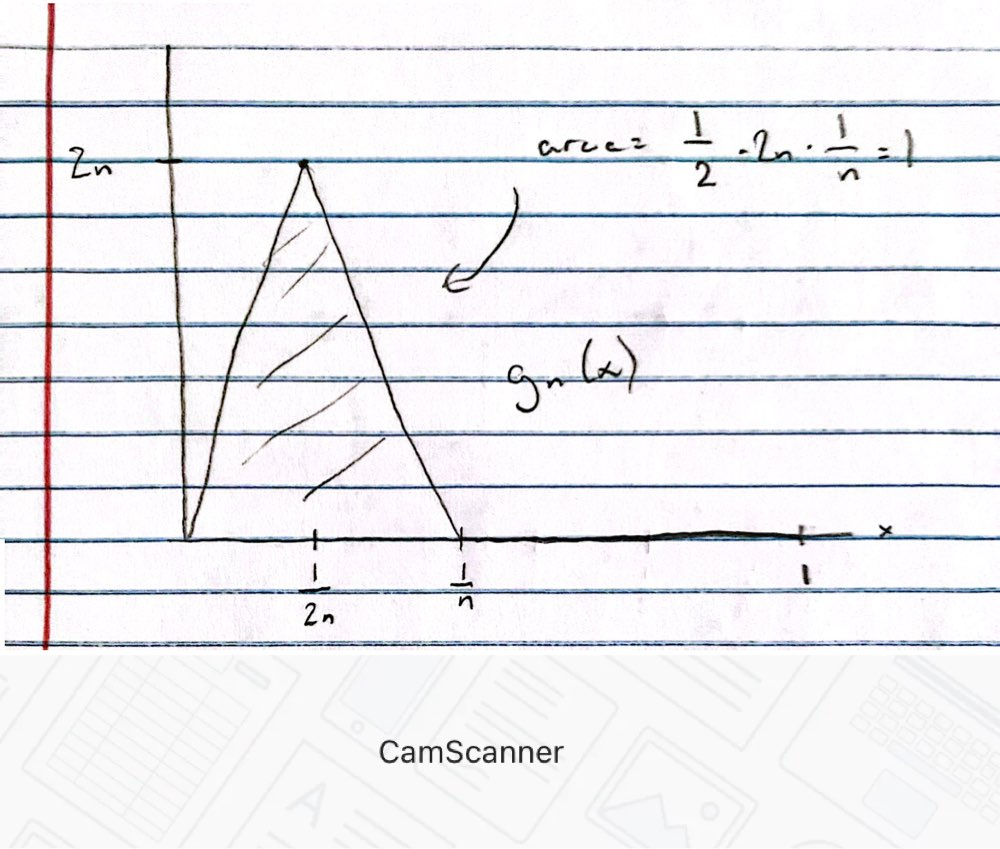
\includegraphics[width = 5in]{Long image 2024-03-10 17.36.49.jpg}
    \end{figure}
    
    
    
    Since $\|f_{n}\|_{2}^{2}=1$, $\|f_{n}\|_{2}=1$ for all $n$. 
\end{proof}

\vspace{0.1 cm}
\item[(b)] Given $n \in \mathbb{N}$, write $n$ in dyadic form,
\begin{equation}
n = 2^j + k ~\mbox{,}
\end{equation}
for $j \in \mathbb{N}_0$ and $0 \leq k \leq 2^j-1$ ; note that both $j$ and $k$ in this decomposition are unique! Define $f_n: [0,1] \to \mathbb{R}$ by
\begin{equation*}
f_n(x) = f_{2^j + k}(x) := \begin{cases} 1 & \mbox{, if } x \in [\frac{k}{2^j},  \frac{k+1}{2^j}]~\mbox{,} \\
                                                    0 & \mbox{, otherwise .} \end{cases}
\end{equation*}

\begin{prop}
    $\|f_n\|_2\to0$ as $n\to\infty$
\end{prop}

\begin{proof}

\begin{lemma}
    $j\to\infty$ as $n\to\infty$
\end{lemma}

\begin{proof}
    Let $M>0$ be given and pick $N$ such that for all $n\ge N$, $$
n\ge 2^{M+1}
$$if 

$$\frac{n}{2}=\frac{2^{j}+k}{2}\le \frac{2^{j}+2^{j}}{2}= 2^{j}$$Therefore, \begin{align*}
j&= \log_{2}(2^{j})\\
&\ge \log_{2}\left(\frac{n}{2}\right)\quad(\log\text{ is monotonic})\\
&\ge \log_{2}\left(\frac{2^{M+1}}{2}\right)\\
&= \log_{2}(2^{M})\\
&= M
\end{align*}
\end{proof}

for $n=2^{j}+k$,  \begin{align*}
    \|f_{n}\|^{2}_{2}&= \int_{0}^{1}\overline{f_{n}(t)}f_{n}(t)\ dt\\
    &= \int_{0}^{1}f_{n}(t)f_{n}(t)\ dt\\
    &= \int_{\frac{k}{2^{j}}}^{\frac{k+1}{2^{j}}}1\ dt\\
    &= \frac{1}{2^{j}}
    \end{align*}Therefore, $f_{n}\rightarrow 0$ in the $L^{2}$ sense as $j \rightarrow \infty$. As $j \rightarrow \infty$ with $n$, $\|f_{n}\|_{2}\rightarrow 0$
    
\end{proof}

\begin{prop}
    For all $x\in[0,1]$, $f_n(x)$ does not converge.
\end{prop}

\begin{proof}
    Fix $x\in[0,1]$. To show that $f_{n}(x)$ does not converge, we show that it is not a Cauchy sequence. This follows from the statement: for all $N\in \mathbb{N}$, there exist $n,m\ge N$ such that $$|f_{n}(x)-f_{m}(x)|=1$$
Let $N\in \mathbb{N}$ be arbitrary and break into two cases: if $x=0$, define \begin{align*}
j_{n}&= N\\
k_{n}&= 0\\
j_{m}&= N\\
k_{m}&= 1\\
n&= 2^{j_n}+k_n=2^N\ge N\\
m&= 2^{j_m}+k_m=2^N+1\ge N
\end{align*}We have $$0\in\left[0, \frac{1}{2^{N}}\right]$$so, $f_{n}(0)=1$, but $$0\notin\left[ \frac{1}{2^{N}},\frac{2}{2^{N}}\right]$$so $f_{m}(0)=0$. Thus, $$|f_{n}(x)-f_{m}(x)|=1$$
For the second case, we take $x>0$. Using the Archimedean law consider an $N$ satisfying $1<2^{N}x$. 

Let $j_{n}=N$ and $$K_{n}=\{k\in \mathbb{N}:k<2^{N}x\}$$Since $1\in K_{n}$ and $K_{n}$ is a set of integers bounded by $2^{N}x$, let $k_{n}=\max K_{n}$. $1\in K_{n}$ implies that $k_{n}\ge1\ge0$. 

Suppose $k_{n}=2^{N}$. Since $k_{n}\le 2^{N}x$, $x=1$. If $k\in K_{n}$, then $k\in \mathbb{N}$ and $k<2^{N}$. So, $k\le2^{N}-1$. This contradicts that $k_{n}$ is an upper bound. Therefore, $k_{n}\ne 2^N$. Since $k\le 2^N$, $k<2^N$. Now, $k\in K_{n}$ implies $k\in \mathbb{N}$ so $k\le2^{N}-1$. This shows that $$n=2^{j_{n}}+k$$is in dyadic form with $$n\ge2^{N}\ge N$$

There $k\in K_{n}$ such that $k+1\ge 2^{N}x$. Otherwise, for all $l\in K_n$, $l+1<2^{N}x$. But, then, $l+1\in K_n$, contradicting that $K_n$ is bounded and nonempty. Thus, $k_{n}\ge k\ge 2^{N}x-1$. So, $$k_{n}\le2^{j_{n}}x\le k_{n}+1$$which implies $$x\in\left[ \frac{k_{n}}{2^{j_{n}}}, \frac{k_{n}+1}{2^{j_{n}}}\right]\iff f_{n}(x)=1$$

Let $j_{m}=2N$ and let $k_{m}=k_{n}-1$. We still have $k_{m}\le 2^{N}-2\le2^{2N}-1=2^{j_{m}}-1$. Thus, $$m=2^{j_{m}}+k_{m}$$is in dyadic form with $$m\ge2^{2N}\ge N$$
We have $$x\ge \frac{k_{n}}{2^{N}}= \frac{k_{m}+1}{2^{N}}> \frac{k_{m}+1}{2^{N}}$$so, $$x\notin\left[\frac{k_{m}}{2^{j_{m}}}, \frac{k_{m}+1}{2^{j_{m}}}\right]\iff f_{m}(x)=0$$
Therefore, \[|f_{n}(x)-f_{m}(x)|=|1-0|=1\]
\end{proof}



\end{itemize}



\end{document}

%------------------------------------------------------------------------------
% End of journal.tex
%------------------------------------------------------------------------------
